\chapter{Supporting Information for the Applications}

\section{Geometries}
The optimised geometries of the molecules discussed in the main paper are deposited at: \href{https://github.com/Crespo-Otero-group/paper_data}{https://github.com/Crespo-Otero-group/paper\_data}
\section{Crystal Structures}
All crystal structures were obtained from the Cambridge Crystallographic Database. The ones available freely are listed in Table \ref{tab:ccdc}. As of writing this paper, $\alpha$MODCS, $\beta$MODCS, $\alpha$MODBDCS, and $\beta$MODBDCS do not have deposited structures.\cite{Shi2019}

\begin{table}[]
    \centering
    \begin{tabular}{ll}
    \toprule
    Crystal & CCDC ID\\\midrule
DSB	& 921998\\
4PV	& 129139\\
HBT	& 727487\\
3P	& 1269382\\
4P	& 1245769\\
6P	& 1319661\\
$\alpha$DCS	& 1247728\\
$\alpha$DBDCS	& 778284\\
$\beta$DBDCS	& 969314\\\bottomrule
    \end{tabular}
    \caption{Cambridge Crystallographic Data Centre (CCDC) IDs for the corresponding crystal structures.}
    \label{tab:ccdc}
\end{table}

\section{Active Space}
CASSCF and CASPT2 were carried out for 3P and HBT. The active spaces are reported in Figure \ref{fig:space}.

\begin{figure}
\centering
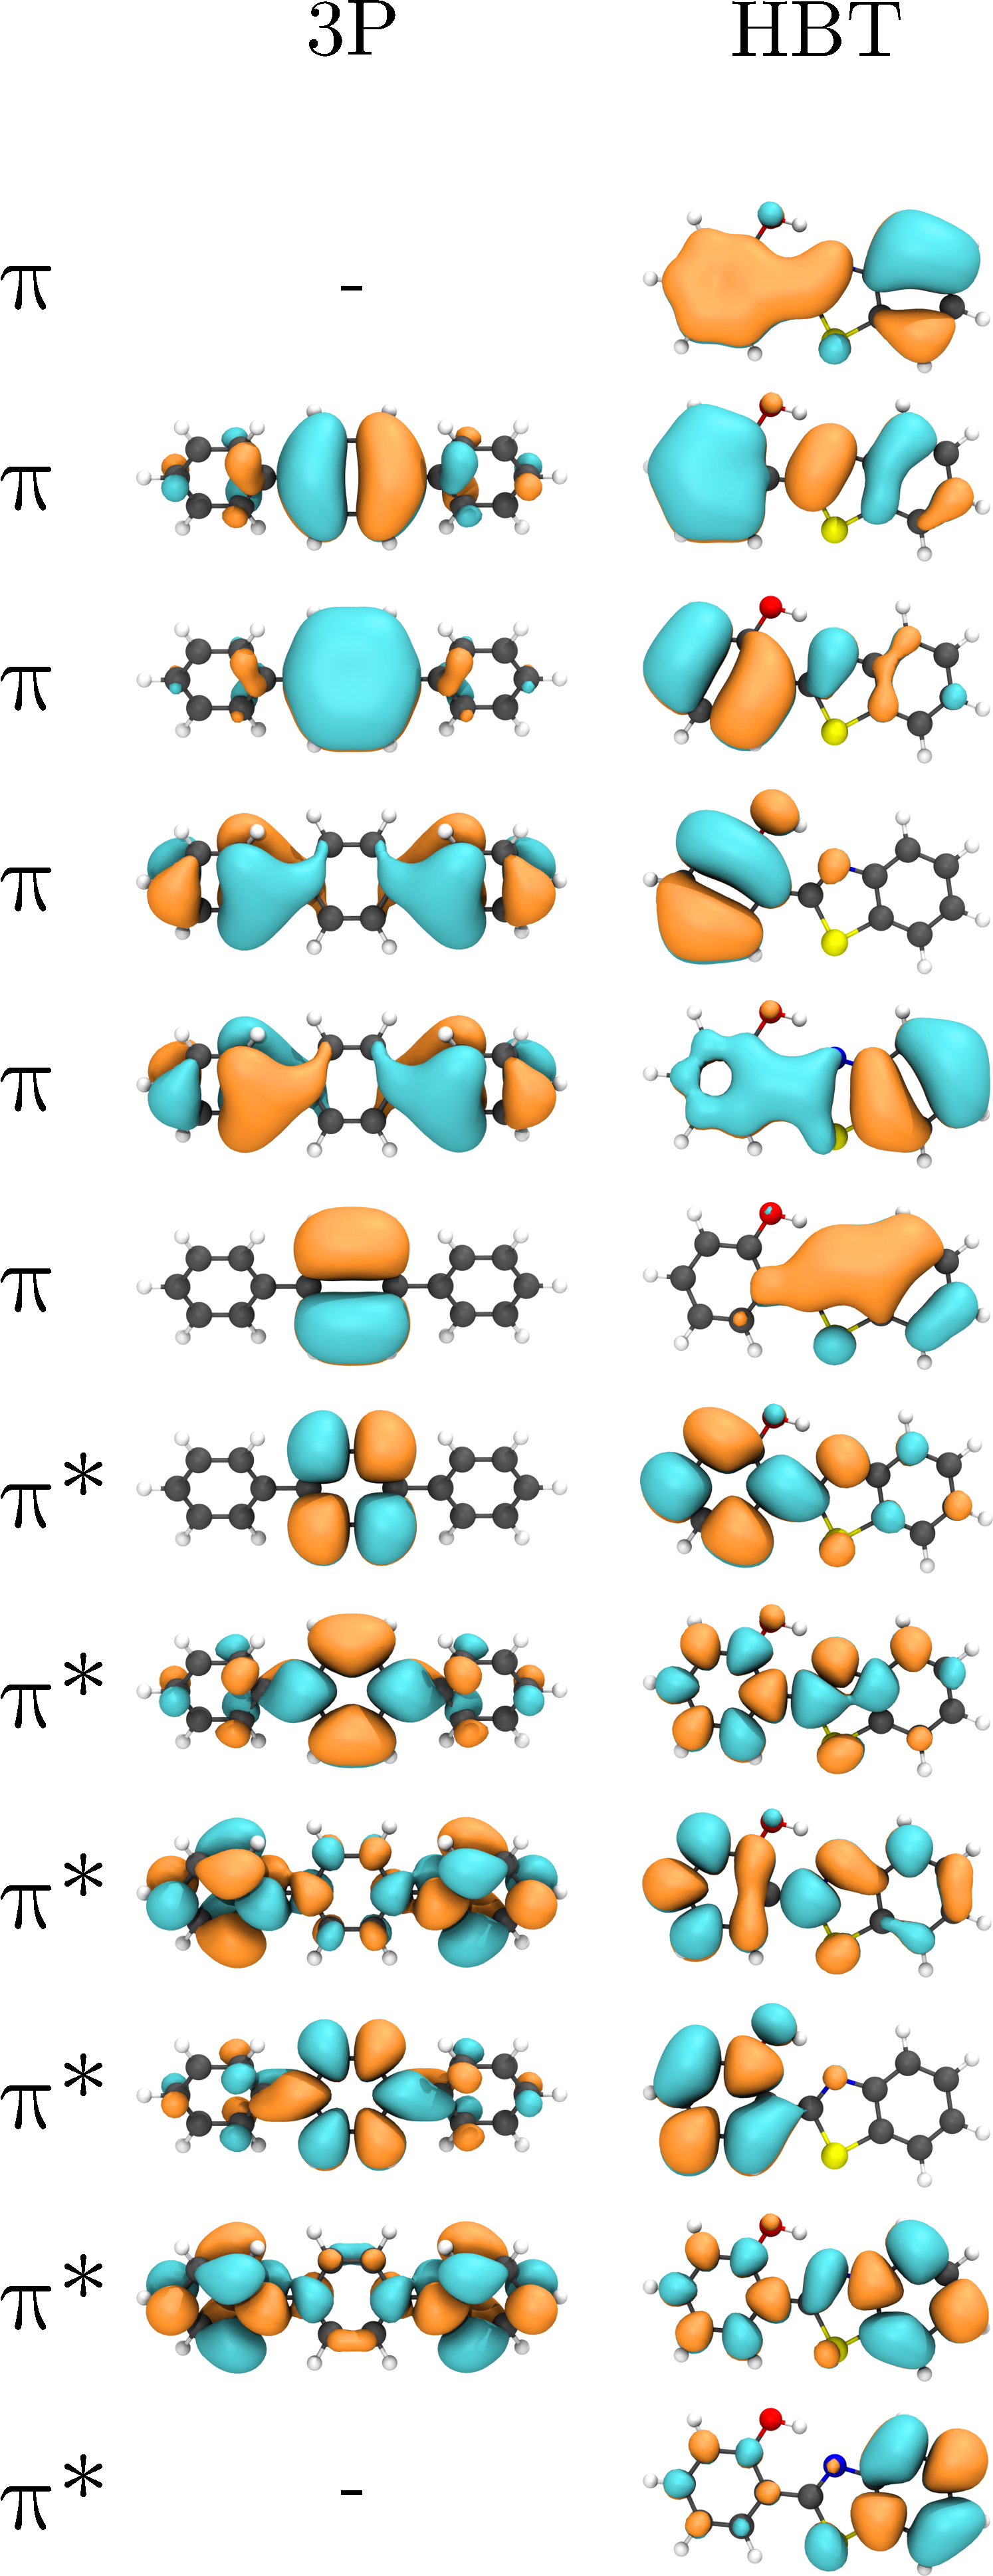
\includegraphics[width=8cm]{Appendices/B/active_spaces.pdf}
\caption{Active spaces of 3P and HBT for multireference calculations.}
\label{fig:space}
\end{figure}

\section{Full Normal Mode Analysis}
The reorganisation energies in vacuum and in crystal discussed in the main paper are only the ones below 250 cm$^{-1}$. Here, we include the rest of the energies:

\begin{table*}[]
\begin{tabular}{@{}lcccccc@{}}
\toprule
\multirow{3}{*}{System} & \multicolumn{6}{c}{Reorganisation energy (cm$^{-1}$)}                                                 \\\cmidrule(lr){2-7}
                        & \multicolumn{3}{c}{Vacuum}                             & \multicolumn{3}{c}{Crystal}             \\\cmidrule(r){1-1} \cmidrule(lr){2-4} \cmidrule(lr){5-7}
                        & $\omega\leq{}250$ & $\omega>250$ & Total  & $\omega\leq{}250$ & $\omega>250$ & Total  \\\midrule
3P                      & 912.7                & 3221.3                 & 4134   & 64.6           & 2791.4        & 2856   \\
4P                      & 1423.7               & 2948.3                 & 4372   & 383.6          & 2560.4        & 2944   \\
6P                      & 912.6                & 3075.4                 & 3988 & 104.3          & 2230.7        & 2335 \\
$\alpha$DCS                  & 764.9                & 2550.1                 & 3315   & 370.7          & 2335.3        & 2706   \\
$\alpha$DBDCS                & 705.9                & 2228.1                 & 2934   & 129.6          & 1916.4        & 2046   \\
$\beta$DBDCS                & 724.6                & 2593.4                 & 3318   & 286.2          & 2672.8        & 2959   \\
$\alpha$MODCS                & 756.2                & 2675.8                 & 3432   & 433.7          & 2013.3        & 2447   \\
$\beta$MODCS                & 721.6                & 1777.4                 & 2499   & 252.3          & 1990.7        & 2243   \\
$\alpha$MODBDCS              & 473.3                & 1971.7                 & 2445   & 71.7           & 1878.3        & 1950   \\
$\beta$MODBDCS              & 617                  & 2106                   & 2723   & 75.6           & 1792.4        & 1868  \\\bottomrule
\end{tabular}
\caption{Reorganisation energies for normal modes of the $n$P and DCS series, in vacuum and crystal, split between low and high energy normal modes.}
\end{table*}

